%!TEX root = ../thesis.tex
%*******************************************************************************
%****************************** Third Chapter **********************************
%*******************************************************************************
\chapter{Diseño Conceptual}

% **************************** Define Graphics Path **************************
\ifpdf
    \graphicspath{{Chapter3/Figuras/}{Chapter3/Figs/PDF/}{Chapter3/Figs/}}
\else
    \graphicspath{{Chapter3/Figs/Vector/}{Chapter3/Figs/}}
\fi

\section{Requerimientos del sistema}
Uno de los requerimientos principales del sistema es el uso de una red de sensores modular y sencilla de instalar en distintos tipos de vehículos. Esto se explica fácilmente debido a que este sistema esta orientado a ser usado en el sistema de transporte público en Lima, el cual tiene una gran variedad y un gran número de vehículos. El sistema, entonces, debe ser adaptable a cualquiera de estos vehículos y no contar con un tiempo de instalación elevado.

También se tiene como requerimiento un grado de precisión alto en el reconocimiento de estilos y eventos de conducción. Esto es necesario debido a que este sistema se usará para monitorizar y mejorar la conducta de conducción de los choferes del servicio de transporte público. Los datos arrojados por este sistema necesitan ser confiables.

Por último, se necesita también de una adecuada infraestructura que permita que el sistema funcione en linea, entregando feedback al conductor, aún si se presentan condiciones como la falta temporal de conexión a Internet. Este requerimiento será importante al considerar donde realizar el procesamiento de los datos (dentro de un sistema embebido en cada vehículo o usando un servidor).


\begin{table}[htbp!]
  \caption{Lista de Requerimientos página 1.}
  \label{diag:3.1}
  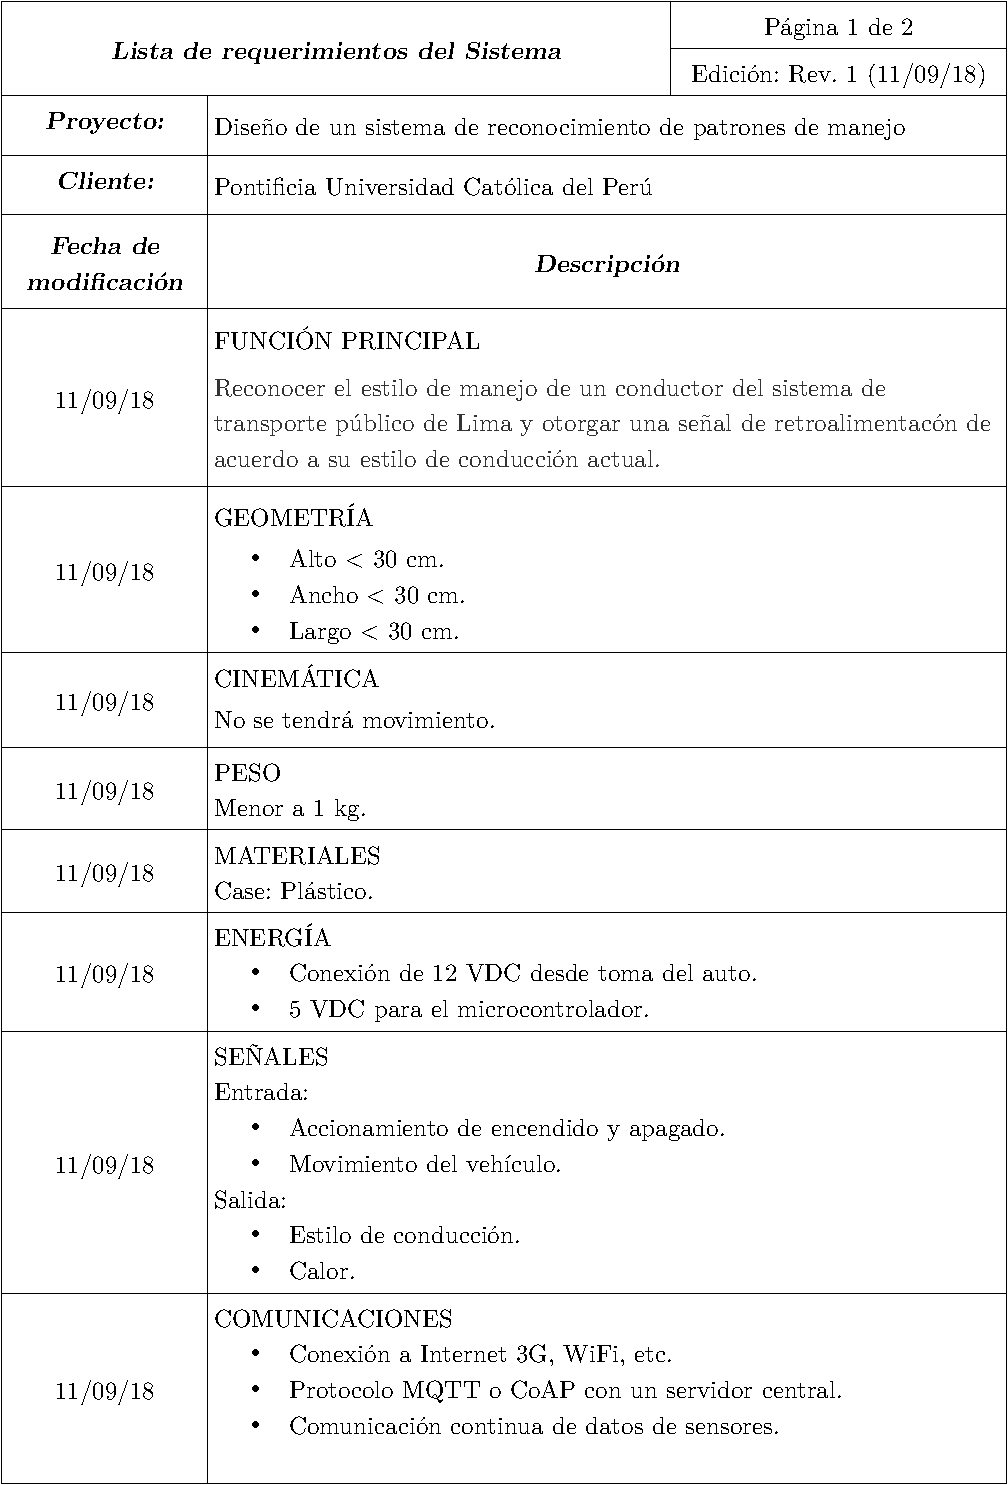
\includegraphics[width=1.05\linewidth]{Tab1.pdf}
\end{table}

\begin{table}[htbp!]
  \caption{Lista de Requerimientos página 2.}
  \label{diag:3.2}
  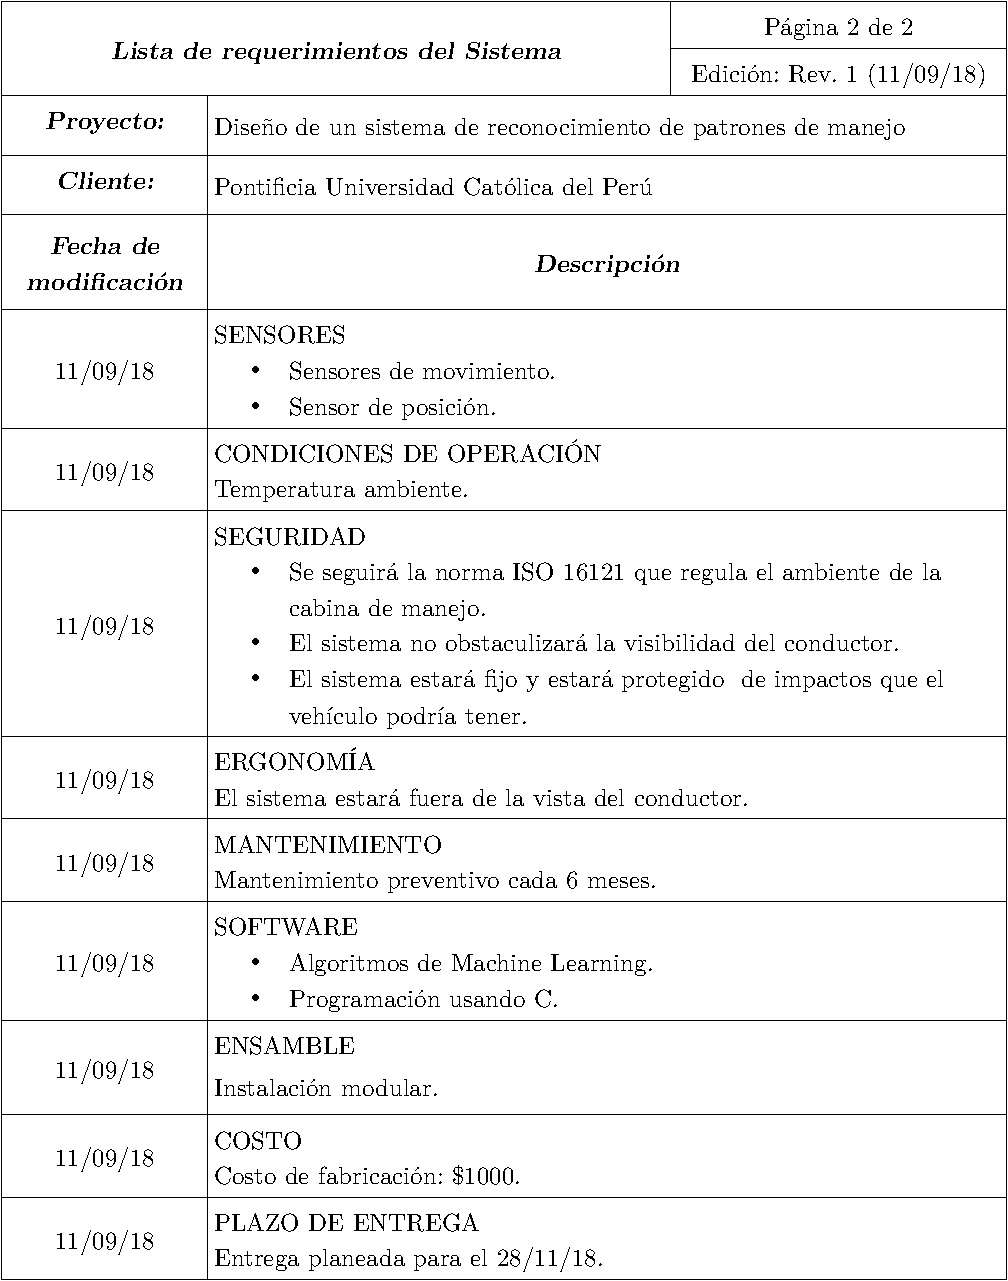
\includegraphics[width=1.05\linewidth]{Tab2.pdf}
\end{table}

\newpage

\section{Modelo Black Box}
En la Fig~\ref{fig:3.1} se puede observar el modelo de Black Box o Caja Negra del sistema. En este modelo se pueden apreciar con mayor claridad las entradas y salidas del sistema

\begin{figure}[htbp!]
\centering
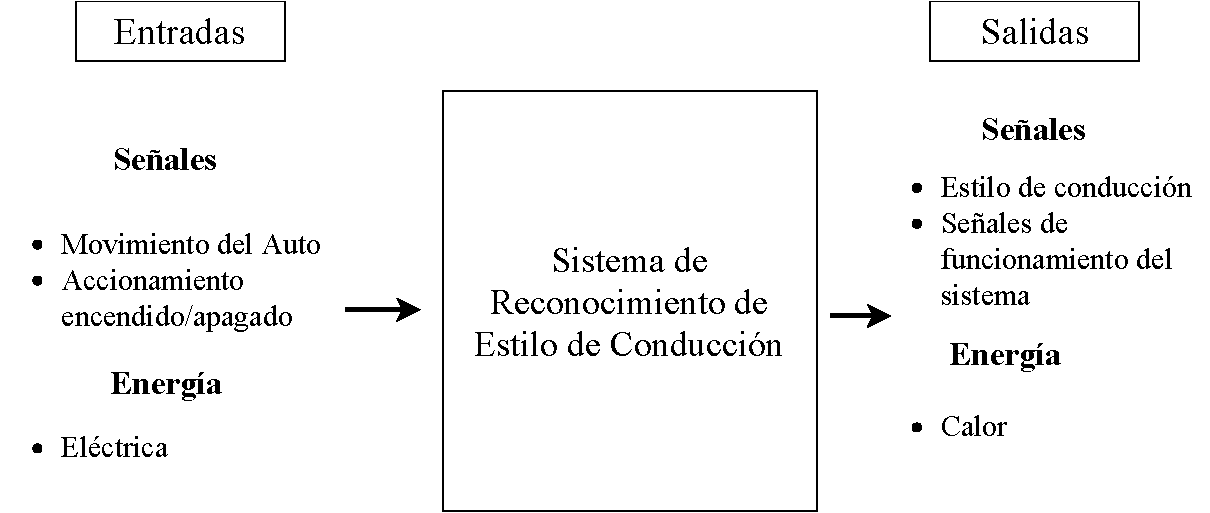
\includegraphics[width=\textwidth]{Fig1.pdf}
\caption{Modelo de Black Box del sistema.}
\label{fig:3.1}
\end{figure}


El sistema estará conectado al auto, de donde obtendrá la energía necesaria para funcionar. Debido a que el enfoque del sistema es ahorrar energía. Su consumo debe ser reducido.

Además de recibir la energía, este sistema procesará el movimiento del auto usando sensores obteniendo así toda la información necesaria para caracterizar el estilo de conducción del usuario. El estilo de conducción será almacenado y será representado como una señal de feedback al usuario. Además el sistema deberá indicar al usuario que se en funcionamiento.

\section{Estructura de Funciones}

\begin{sidewaysfigure}[htbp!]
\centering
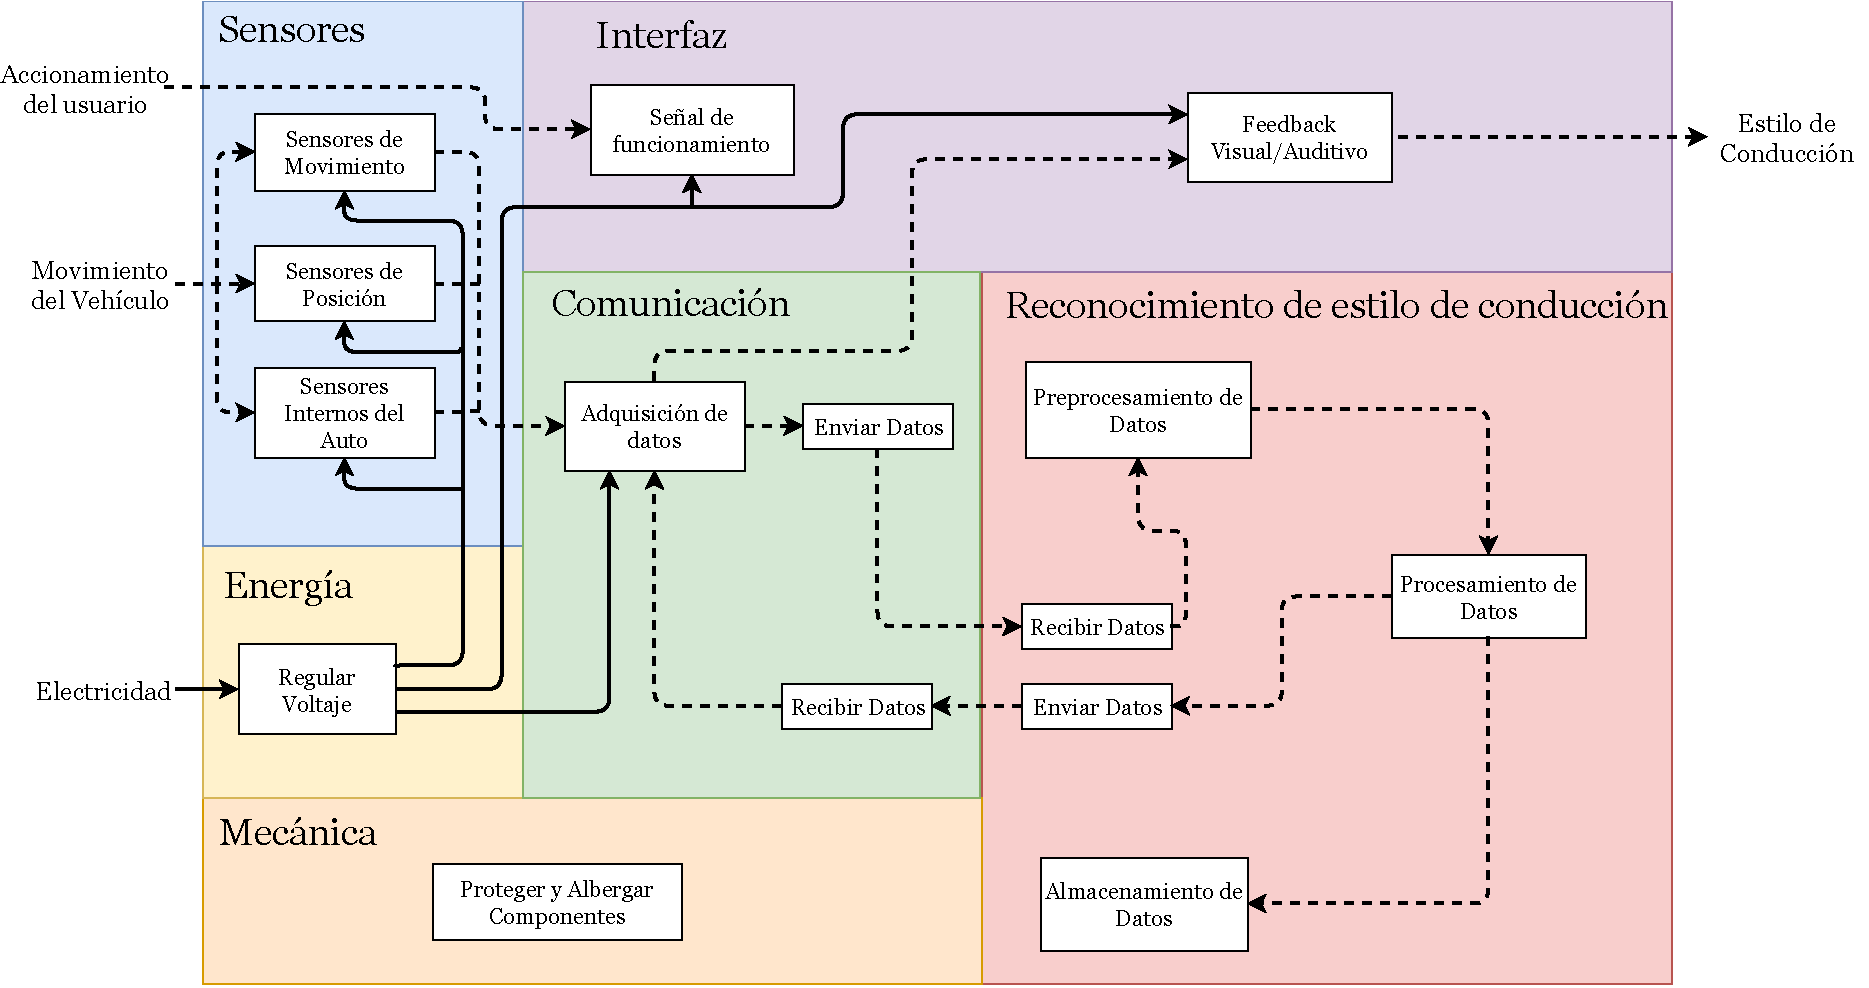
\includegraphics[width=\textwidth]{Tab3.pdf}
\caption{Estructura de Funciones.}
\label{fig:3.2}
\end{sidewaysfigure}

La estructura de funciones del sistema se puede apreciar en la Fig~\ref{fig:3.2}. Para el elaboramiento de esta se han considerado 6 módulos: Mecánica, Energía, Sensores, Comunicación, Reconocimiento del estilo de conducción e Interfaz.

Se describirá a continuación cada uno de estos módulos para así obtener una visión general del funcionamiento total del sistema.

\subsection{Módulo mecánico}
En este módulo Fig~\ref{fig:3.3} se encuentra la  función de proteger y albergar todos los componentes del sistema. Se debe tener en cuenta que la velocidad relativa entre el vehículo y el sistema debe ser nula para que las medidas de los sensores sean precisas.

Además es importante también proteger al sistema de elementos como el polvo y la humedad. Por lo que se ejercerá la función de proteger al sistema.

\begin{figure}[htbp!]
\centering
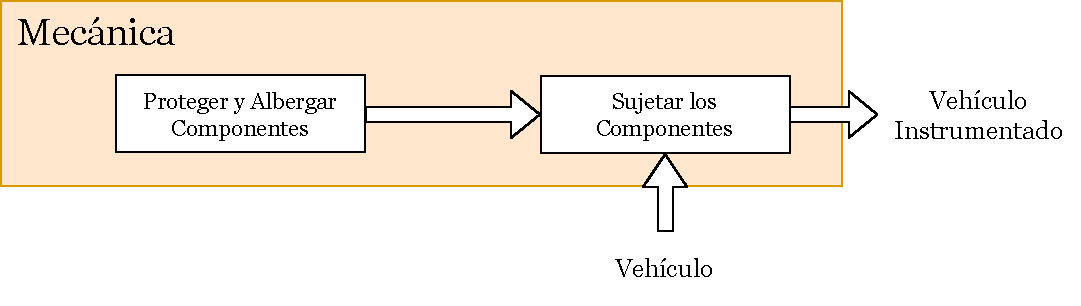
\includegraphics[width=0.8\textwidth]{mec.pdf}
\caption{Módulo mecánico de la estructura de funciones.}
\label{fig:3.3}
\end{figure}

\subsection{Módulo de energía}
Este módulo Fig~\ref{fig:3.4} cumplirá la función de obtener la energía eléctrica necesaria para el funcionamiento del sistema y regular el voltaje, entregándole a cada módulo esta energía según sus requerimientos específicos. Los módulos que recibirán la energía serán los de Comunicación, Sensores e Interfaz.

\begin{figure}[htbp!]
\centering
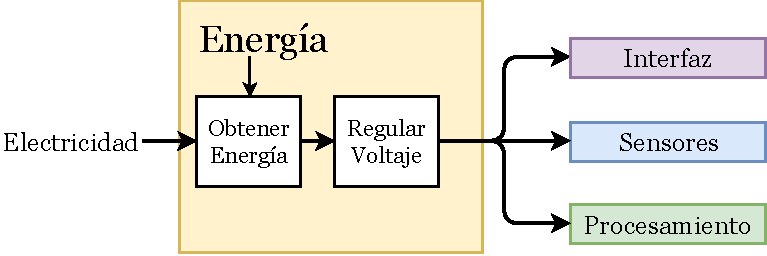
\includegraphics[width=0.6\textwidth]{elec.pdf}
\caption{Módulo eléctrico de la estructura de funciones.}
\label{fig:3.4}
\end{figure}


\subsection{Módulo de sensores}
Este módulo Fig~\ref{fig:3.5} realizará la función de recibir la información del movimiento del vehículo y transmitir esa información al módulo de comunicaciones que adquirirá todos los datos. Estos sensores serán tanto de movimiento, como de posición, pero además de estos se usarán los sensores internos del vehículo si estos se encuentran disponibles.

\begin{figure}[htbp!]
\centering
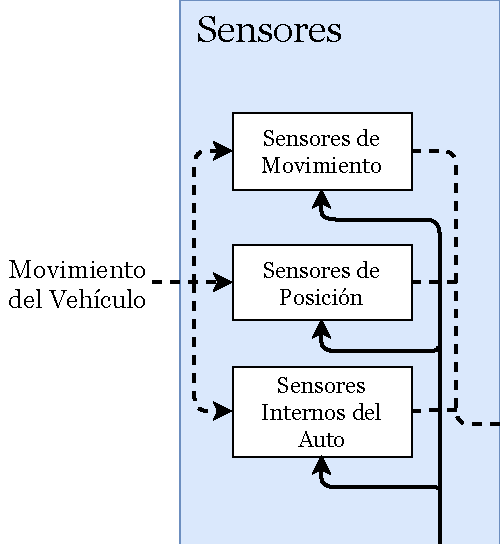
\includegraphics[width=0.5\textwidth]{sens.pdf}
\caption{Módulo de sensores de la estructura de funciones.}
\label{fig:3.5}
\end{figure}

\subsection{Módulo de comunicación}
En este módulo Fig~\ref{fig:3.6} se ejecutarán las funciones de adquirir los datos que el módulo de sensores entrega. Luego de adquirirlos, se necesita enviar estos datos para su procesamiento y recibirlos una vez estén procesados. Los datos procesados representarán al estilo de manejo del conductor, por lo que esta información será entregada al módulo de interfaz para que sean mostrados al usuario.

\begin{figure}[htbp!]
\centering
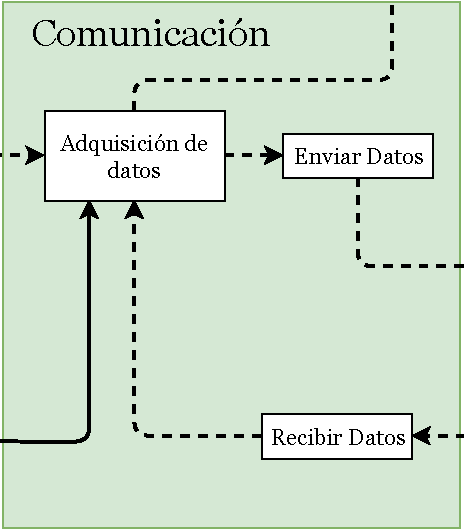
\includegraphics[width=0.5\textwidth]{com.pdf}
\caption{Módulo de comunicación de la estructura de funciones.}
\label{fig:3.6}
\end{figure}


\subsection{Módulo de reconocimiento de estilo de conducción}
En este módulo se realizará el procesamiento de la data que fue enviada por el MCU. Para realizar esto se realizará un preprocesamiento de la data para luego procesarla usando algoritmos de machine learning.

\begin{figure}[htbp!]
\centering
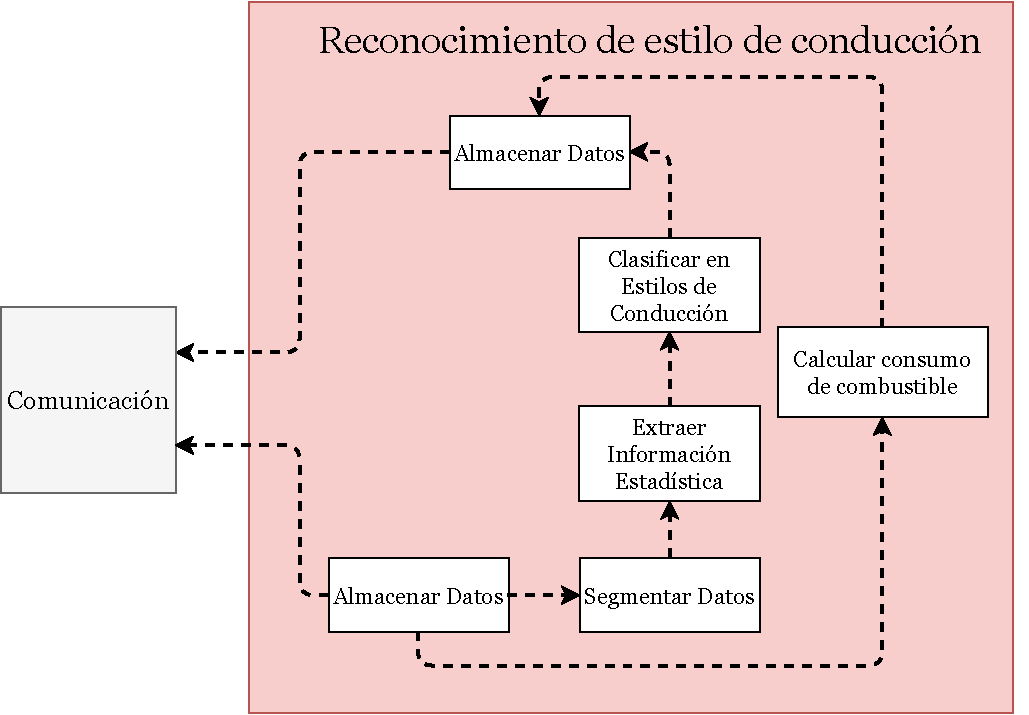
\includegraphics[width=0.6\textwidth]{rec.pdf}
\caption{Módulo de reconocimiento de estilo de conducción de la estructura de funciones.}
\label{fig:3.7}
\end{figure}

Cuando la data haya sido procesada, se tendrá el estilo de conducción resultante que será enviado de vuelta al MCU por el servidor. Sin embargo, la data usada para obtener este resultado se conservará. Esta data se almacenará en el servidor para poder hacer análisis offline o implementar otros servicios que puedan hacer uso de la información disponible, como un seguimiento en tiempo real de los buses, un monitoreo de los conductores, etc.
